\subsection{Цель выполнения лабораторной работы}\label{blockN.VariantM}
\textbf{Цель выполнения лабораторной работы }-- \GoalOfResearch

%-------------------------------------------------
\subsection{Задание}

Решить с помощью МКЭ уравнение \ref{usl}
\begin{align}\label{usl}
1\frac{d^2u}{dx^2}    -15   u  + 4 
=0,
\end{align}
при следующих граничных условиях (г. у.): 
\begin{align}\label{2_rod}
    u(x=3) = 10,
\end{align}
\begin{align}\label{1_rod}
    u'(x=14) = 1.
\end{align}

Количество конечных элементов
\begin{itemize}
    \item для первого расчета -- 20,
    \item для второго -- 40.
\end{itemize}

Также необходимо:
\begin{enumerate}
    \item Сравнить результаты с аналитическим решением. Оценить максимальную погрешность.
    \item Определить количество линейных КЭ, обеспечивающих такую же точность как и кубические.
\end{enumerate}

%-------------------------------------------------
\newpage
\subsection{Аналитическое решение}

На рисунке \ref{analit} представлено аналитическое решение поставленной задачи.
\begin{figure}[!h]
\begin{center}
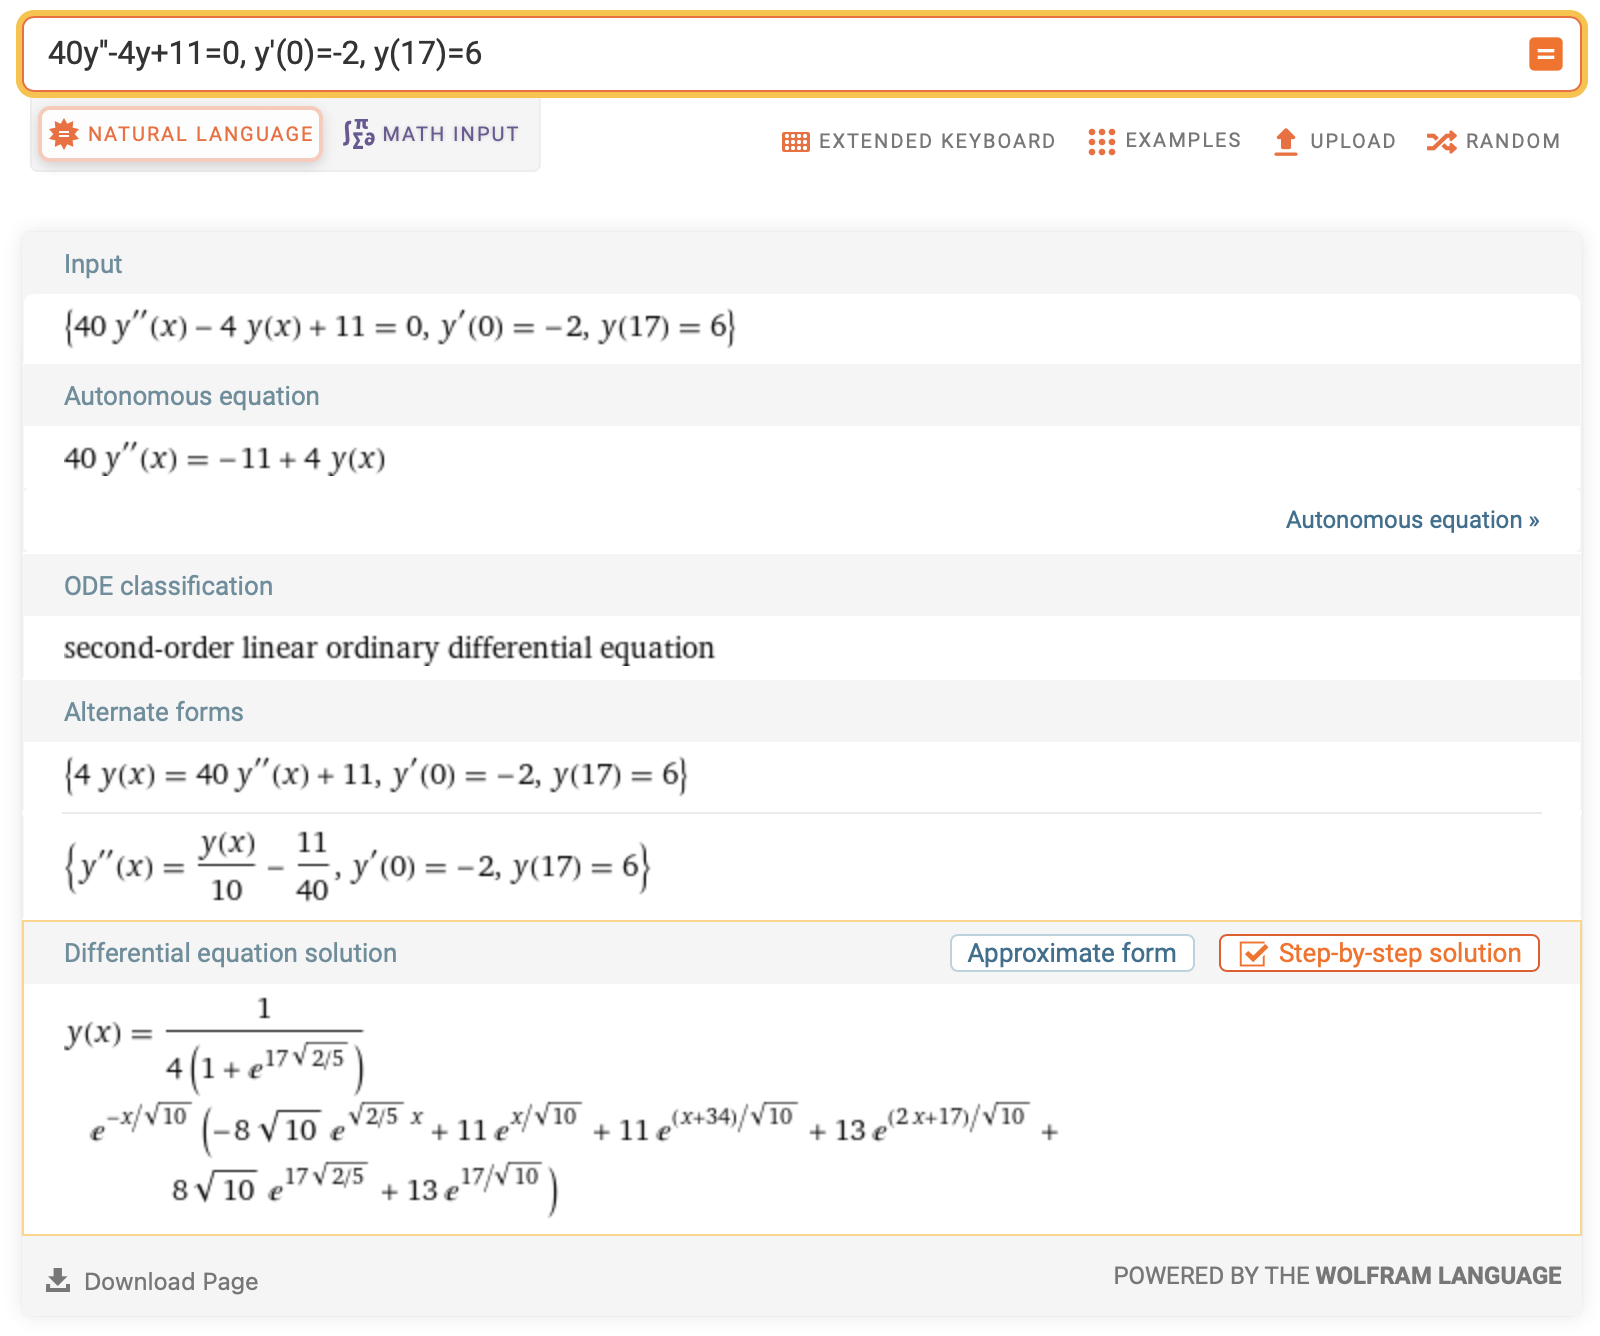
\includegraphics[scale = 0.5]{labs/img/img1}
\end{center}
\caption{Аналитическое решение}
\label{analit}
\end{figure}

Таким образом, получаем:
$$
u(x)=\begin{multline}\frac{1}{15\left(1+e^{22 \sqrt{15}}\right)} \\ e^{-\sqrt{15}(x+3)}\left(146 e^{2 \sqrt{15} x}+4 e^{\sqrt{15}(x+3)}+4 e^{\sqrt{15}(x+25)}+\sqrt{15} e^{\sqrt{15}(2 x+11)}-\right. \left.\quad \sqrt{15} e^{17 \sqrt{15}}+146 e^{28 \sqrt{15}}\right)\end{multline}.
$$


\subsection{Получение локальных матрицы жесткости и вектора нагрузок}

Составим локальные матрицу жесткости и вектор нагрузок для уравнения \ref{usl}.

\subsubsection{Линейная функция-формы КЭ}

$$
\mathbf{u}=\begin{bmatrix}
(1-\frac{x}{L}) ; & \frac{x}{L}
\end{bmatrix}
\begin{bmatrix}
u_i \\
u_j
\end{bmatrix}
=\mathbf{N_eU},
$$
где $\mathbf{N_e}$ -- вектор функции формы конечного элемента (в данном случае линейной), его составляющие элементы - глобальные базисные функции, отличные от нуля в пределах этого элемента, $L$ -- длина КЭ.

В соответствии с методом Галеркина для уравнения \ref{usl}:
\begin{equation}\label{lin}
\int_0^L \mathbf{W_e}\left( 1\frac{d^2\mathbf{u}}{dx^2} \frac{d\mathbf{u}}{dx}  +4 \right) d x=0,
\end{equation}
где $\mathbf{W_e=N_e}^T$.

$$\int_0^L \mathbf{W_e}\left(1\frac{d^2\mathbf{u}}{dx^2} \frac{du}{dx}  +4 \right) d x= 1\int_0^L \mathbf{W_e} \frac{d^2 \mathbf{u}}{dx^2} dx   \int_0^L \mathbf{W_e}\frac{d\mathbf{u}}{dx} d x   +4 \int_0^L \mathbf{W_e} d x=0$$

Распишем каждое слагаемое отдельно:
$$
1\int_0^L \mathbf{W_e} \frac{d^2 \mathbf{u}}{dx^2} dx=1\int_0^L
	\begin{bmatrix}
	(1-\frac{x}{L}) \\
	\frac{x}{L}
	\end{bmatrix}
\frac{d^2 \mathbf{u}}{dx^2} dx =
1
	\begin{bmatrix}
	(1-\frac{x}{L}) \\
	\frac{x}{L}
	\end{bmatrix}
\frac{d\mathbf{u}}{dx} |_0^L -
$$
$$
  -1  \int_0^L
\frac{d}{dx}
	\begin{bmatrix}
	(1-\frac{x}{L}) \\
	\frac{x}{L}
	\end{bmatrix}
\frac{d}{dx}
	\begin{bmatrix}
	(1-\frac{x}{L}); & \frac{x}{L}
	\end{bmatrix}
	\begin{bmatrix}
	u_i \\
	u_j
	\end{bmatrix}
=
	\begin{bmatrix}
	  -1 \frac{d\mathbf{u}}{dx}|_i \\
1\frac{d\mathbf{u}}{dx}|_j
	\end{bmatrix}   -1 
\begin{bmatrix}
\frac{1}{L}, & -\frac{1}{L} \\
-\frac{1}{L}, & \frac{1}{L}
\end{bmatrix}
\begin{bmatrix}
u_i \\
u_j
\end{bmatrix}
$$

$$
 \int_0^L \mathbf{W_e} \frac{d \mathbf{u}}{dx} dx= \int_0^L
	\begin{bmatrix}
	(1-\frac{x}{L}) \\
	\frac{x}{L}
	\end{bmatrix}
\frac{d \mathbf{u}}{dx}
	\begin{bmatrix}
	u_i \\
	u_j
	\end{bmatrix}
dx
=
$$
$$
=
 
\int_0^L
\begin{bmatrix}
	(1-\frac{x}{L}) & (-1+\frac{x}{L})\\
	-\frac{x}{L} & \frac{x}{L}
\end{bmatrix}
\begin{bmatrix}
	u_i \\
	u_j
\end{bmatrix}
=
 
\begin{bmatrix}
-\frac{1}{2}, & \frac{1}{2} \\
-\frac{1}{2}, & \frac{1}{2}
\end{bmatrix}
\begin{bmatrix}
u_i \\
u_j
\end{bmatrix}
$$

$$4\int_0^L \mathbf{W_e} d x= 4
\begin{bmatrix}
	\frac{L}{2} \\
	\frac{L}{2}
\end{bmatrix}
$$

Таким образом, для уравнения \ref{lin}, при использовании линейной функции-формы,  получаем (матмодель линейного КЭ):

$$
\begin{bmatrix}
	1\frac{1}{L}   \frac{1}{2}, &   -1 \frac{1}{L}   \frac{1}{2} \\
	  -1  \frac{1}{L}  \frac{1}{2}, &  1\frac{1}{L}   \frac{1}{2}
\end{bmatrix}
\begin{bmatrix}
	u_i \\
	u_j
\end{bmatrix}=
\begin{bmatrix}
	  -1 \frac{du}{dx}|_i   +4  \frac{L}{2}\\
	1\frac{du}{dx}|_j   +4  \frac{L}{2}
\end{bmatrix}
$$


\subsubsection{Кубическая функция-формы КЭ}
$$
\mathbf{u}=\begin{bmatrix}
-\frac{9x^3}{2L^3}+\frac{18x^2}{2L^2}-\frac{11x}{2L} + 1;
\frac{27x^3}{2L^3}-\frac{45x^2}{2L^2}+\frac{9x}{L};
-\frac{27x^3}{2L^3}+\frac{36x^2}{2L^2}-\frac{9x}{2L};
\frac{9x^3}{2L^3}-\frac{9x^2}{2L^2}-\frac{x}{L};
\end{bmatrix}
\begin{bmatrix}
u_i \\
u_j\\
u_k\\
u_l
\end{bmatrix}
=\mathbf{N_eU},
$$

Как и для линейной функции-формы применим метод Галеркина (см. уравнение \ref{lin}) и рассмотрим каждое слагаемое отдельно.

$$1 \int_0^L \mathbf{W_e} \frac{d^2 \mathbf{u}}{dx^2} dx
=
1\int_0^L
\begin{bmatrix}
	-\frac{9x^3}{2L^3}&+&\frac{18x^2}{2L^2}&-&\frac{11x}{2L} &+& 1\\
	\frac{27x^3}{2L^3}&-&\frac{45x^2}{2L^2}&+&\frac{9x}{L}&&\\
	-\frac{27x^3}{2L^3}&+&\frac{36x^2}{2L^2}&-&\frac{9x}{2L}&&\\
	\frac{9x^3}{2L^3}&-&\frac{9x^2}{2L^2}&-&\frac{x}{L}&&
\end{bmatrix}
\frac{d^2 \mathbf{u}}{dx^2} dx
=
$$
$$
=
1
\begin{bmatrix}
	-\frac{9x^3}{2L^3}&+&\frac{18x^2}{2L^2}&-&\frac{11x}{2L} &+& 1\\
	\frac{27x^3}{2L^3}&-&\frac{45x^2}{2L^2}&+&\frac{9x}{L}&&\\
	-\frac{27x^3}{2L^3}&+&\frac{36x^2}{2L^2}&-&\frac{9x}{2L}&&\\
	\frac{9x^3}{2L^3}&-&\frac{9x^2}{2L^2}&-&\frac{x}{L}&&
\end{bmatrix}
\frac{d\mathbf{u}}{dx} |_0^L
  -1  \int_0^L \frac{d}{dx}
\begin{bmatrix}
	-\frac{9x^3}{2L^3}&+&\frac{18x^2}{2L^2}&-&\frac{11x}{2L} &+& 1\\
	\frac{27x^3}{2L^3}&-&\frac{45x^2}{2L^2}&+&\frac{9x}{L}&&\\
	-\frac{27x^3}{2L^3}&+&\frac{36x^2}{2L^2}&-&\frac{9x}{2L}&&\\
	\frac{9x^3}{2L^3}&-&\frac{9x^2}{2L^2}&-&\frac{x}{L}&&
\end{bmatrix}
\frac{d}{dx} \mathbf{u}
=$$
$$
=
\begin{bmatrix}
	  -1 \frac{d\mathbf{u}}{dx}|_i \\
	0\\
	0\\
1\frac{d\mathbf{u}}{dx}|_l
\end{bmatrix}
  -1 
\begin{bmatrix}
\begin{array}{rrrr}
	\frac{37}{10L} & -\frac{189}{40} & \frac{27}{20L} & -\frac{13}{40L}\\
	-\frac{189}{40} & \frac{54}{5L} & -\frac{297}{40L} & \frac{27}{20L}\\
	\frac{27}{20L} &  -\frac{297}{40L} & \frac{54}{5L} & -\frac{189}{40}\\
	-\frac{13}{40L} & \frac{27}{20L} & -\frac{189}{40} & \frac{37}{10L}
\end{array}
\end{bmatrix}
\begin{bmatrix}
u_i \\
u_j \\
u_k\\
u_l
\end{bmatrix}
$$

$$
  \int_0^L \mathbf{W_e} \frac{d \mathbf{u}}{dx} dx
=
 \int_0^L
\begin{bmatrix}
  -\frac{9x^3}{2L^3}&+&\frac{18x^2}{2L^2}&-&\frac{11x}{2L} &+& 1\\
  \frac{27x^3}{2L^3}&-&\frac{45x^2}{2L^2}&+&\frac{9x}{L}&&\\
  -\frac{27x^3}{2L^3}&+&\frac{36x^2}{2L^2}&-&\frac{9x}{2L}&&\\
  \frac{9x^3}{2L^3}&-&\frac{9x^2}{2L^2}&-&\frac{x}{L}&&
\end{bmatrix}
\frac{d \mathbf{u}}{dx} dx
=
$$
$$
=
 
\begin{bmatrix}
\begin{array}{rrrr}
	-\frac{1}{2} & \frac{57}{80} & -\frac{3}{10} & \frac{7}{80}\\
	-\frac{57}{80} & 0 & \frac{81}{80} & -\frac{3}{10} \\
	\frac{3}{10} & -\frac{81}{80} & 0 & -\frac{3}{10}\\
	-\frac{7}{80} & \frac{3}{10} & -\frac{57}{80} & \frac{1}{2}
\end{array}
\end{bmatrix}
\begin{bmatrix}
	u_i \\
	u_j \\
	u_k\\
	u_l
\end{bmatrix}
$$

$$
4 \int_0^L \mathbf{W_e} d x
=
4
\begin{bmatrix}
	\frac{L}{8} \\
	\frac{3L}{8}\\
	\frac{3L}{8}\\
	\frac{L}{8}
\end{bmatrix}
$$

\newpage
Таким образом, для уравнения \ref{lin}, при использовании кубической функции-формы,  получаем:

\begin{align}\label{cub}
\begin{bmatrix}1\frac{37}{10L} \frac{1}{2} &   -1 \frac{189}{40L} \frac{57}{80} & 1\frac{27}{20L} \frac{3}{10} &   -1 \frac{13}{40L}   \frac{7}{80}\\
	  -1 \frac{189}{40L}  \frac{57}{80} & 1\frac{54}{5L}+0 &   -1 \frac{297}{40L} \frac{81}{80} & 1\frac{27}{20L}  \frac{3}{10} \\
	1\frac{27}{20L}   \frac{3}{10} &   -1 \frac{297}{40L} \frac{81}{80} & 1\frac{54}{5L}+0 &   -1 \frac{189}{40L}  \frac{57}{80} \\
	  -1 \frac{13}{40L}  \frac{7}{80} & 1\frac{27}{20L} \frac{3}{10} &   -1 \frac{189}{40L} \frac{57}{80} & 1\frac{37}{10L}  \frac{1}{2}
\end{bmatrix}
\begin{bmatrix}
	u_i \\
	u_j \\
	u_k\\
	u_l
\end{bmatrix}
=
\begin{bmatrix}
    4\frac{L}{8}   -1  \frac{du}{dx}|_i \\
	4\frac{3L}{8}\\
	4\frac{3L}{8}\\
	4\frac{L}{8}   +1  \frac{du}{dx}|_l
\end{bmatrix}
\end{align}

Локальные матрицу жесткости и вектор нагрузок из уравнения \ref{cub} с помощью матричных преобразований приведем к следующему виду:

$$ \begin{bmatrix}
a_{11}     &  0  & 0  &  a_{14}\\
a_{21}     &  a_{22}  & 0  &  a_{24}\\
a_{31}     &  0  &  a_{33} &  a_{34}\\
a_{41}     &  0  & 0  &  a_{44}
\end{bmatrix}
\begin{bmatrix}
u_i \\
u_j \\
u_k\\
u_l
\end{bmatrix} =
\begin{bmatrix}
b_1   -1  \frac{du}{dx}|_i \\
b_2\\
b_3\\
b_4   +1  \frac{du}{dx}|_l
\end{bmatrix}$$

Для упрощения расчетов преобразуем систему выше, исключив внутренние узлы. Таким образом СЛАУ (математическая модель кубического КЭ):

$$ \begin{bmatrix}
a_{11}     &   a_{14}\\
a_{41}     &    a_{44}
\end{bmatrix}
\begin{bmatrix}
u_i \\
u_l
\end{bmatrix} =
\begin{bmatrix}
b_1   -1  \frac{du}{dx}|_i \\
b_4   +1  \frac{du}{dx}|_l
\end{bmatrix}$$

%-------------------------------------------------
\subsection{Получение глобальных матрицы жесткости и вектора нагрузок}

Проведем процедуры ансамблирования и учет граничных условий для формирования итоговой математической модели.

\subsubsection{Ансамблирование}

Пусть локальные матрица жесткости и вектор неизвестных заданы следующим образом

$$
\begin{bmatrix}
a_{11}     &   a_{12}\\
a_{21}     &    a_{22}
\end{bmatrix}
\begin{bmatrix}
u_i \\
u_j
\end{bmatrix} =
\begin{bmatrix}
b_1   -1  \frac{du}{dx}|_i \\
b_2   +1  \frac{du}{dx}|_l
\end{bmatrix},$$

тогда, при разбитие области на $n$ КЭ, глобальная матрица жесткости  будет иметь размерность $(n+1)\cdot(n+1)$:

$$ \begin{bmatrix}
a_{11}^1     &   a_{12}^1         &   0 & \cdots & 0 & 0 & 0  & 0\\
a_{21}^1     &    a_{22}^1+a_{11}^2 & a_{12}^2  & 0 & \cdots & 0 & 0  & 0\\
0     &    a_{21}^2 & a_{22}^2+a_{11}^3  &  a_{12}^3  & 0 & \cdots & 0  & 0\\
0     &    0  & a_{21}^3  & a_{22}^3+ \cdots  &  & &   & 0\\
\vdots & \vdots & \vdots & \vdots &  &  &   & \vdots\\
0 & 0 & 0 & 0 &  0 & 0 & \cdots+a_{11}^n  & a_{12}^n\\
0 & 0 & 0 & 0 &  0 & 0 & a_{21}^n  & a_{22}^n
\end{bmatrix}
\begin{bmatrix}
u_0 \\
u_1 \\
u_2\\
u_3\\
\vdots\\
u_{n-1}\\
u_n
\end{bmatrix} =
\begin{bmatrix}
b_1^1   -1  \frac{du}{dx}|_0 \\
b_2^1+b_1^2\\
b_2^2+b_1^3\\
b_2^3+b_1^4\\
\vdots\\
b_2^{n-1}+b_1^n\\
b_2^n   +1  \frac{du}{dx}|_L
\end{bmatrix}
$$

\subsubsection{Учет граничных условий}

Применим граничные условия первого (см. \ref{1_rod}) и второго рода (см. \ref{2_rod}) к выведенной выше системе.

$$
\begin{bmatrix}
1     &   0        &   0 & \cdots & 0 & 0 & 0  & 0\\
a_{21}^1     &    a_{22}^1+a_{11}^2 & a_{12}^2  & 0 & \cdots & 0 & 0  & 0\\
0     &    a_{21}^2 & a_{22}^2+a_{11}^3  &  a_{12}^3  & 0 & \cdots & 0  & 0\\
0     &    0  & a_{21}^3  & a_{22}^3+ \cdots  &  & &   & 0\\
\vdots & \vdots & \vdots & \vdots &  &  &   & \vdots\\
0 & 0 & 0 & 0 &  0 & 0 & \cdots+a_{11}^n  & a_{12}^n\\
0 & 0 & 0 & 0 &  0 & 0 & 0 & 1
\end{bmatrix}
\begin{bmatrix}
u_0 \\
u_1 \\
u_2\\
u_3\\
\vdots\\
u_{n-1}\\
u_n
\end{bmatrix} =
\begin{bmatrix}
 10   \\
b_2^1+b_1^2\\
b_2^2+b_1^3\\
b_2^3+b_1^4\\
\vdots\\
b_2^{n-1}+b_1^n\\
 b_2^n   +1  \cdot 1   \\
\end{bmatrix}
$$

\subsection{Анализ результатов}

Проведем сравнение результатов согласно заданию.

\subsubsection{Линейная функция-формы}


На рисунках \ref{l_20}, \ref{l_40} представлены графики полученные с помощью МКЭ (линейная функция-формы).

\begin{figure}[!h]
    \centering
    \begin{minipage}{0.5\textwidth}
        \centering
        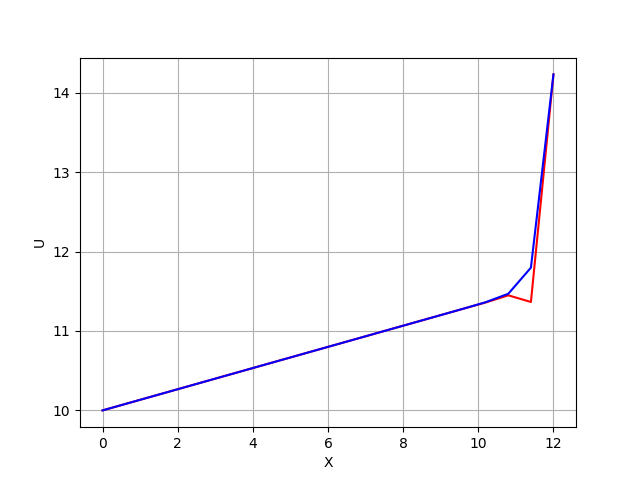
\includegraphics[width=1\textwidth]{labs/img/lin/20.png} % первое изображениие
        \caption{Результат работы программы для 20 КЭ}
        \label{l_20}
    \end{minipage}\hfill
    \begin{minipage}{0.5\textwidth}
        \centering
        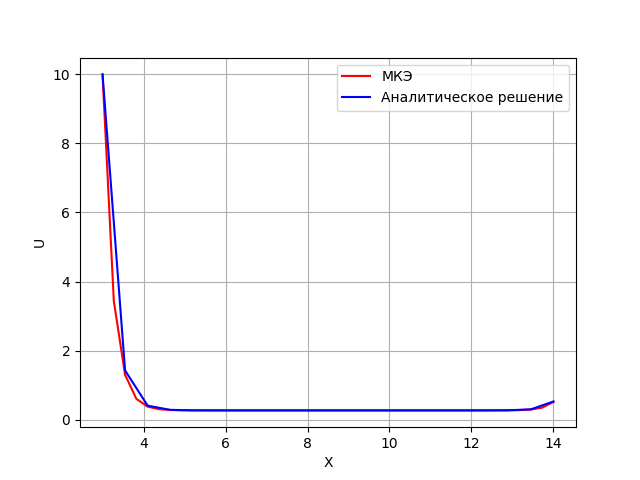
\includegraphics[width=1\textwidth]{labs/img/lin/40.png} % второе изображение
        \caption{Результат работы программы для 40 КЭ}
        \label{l_40}
    \end{minipage}
\end{figure}

\begin{table}[H]
\centering
\begin{tabular}{|c|c|c|c|}
\hline
X & Аналитическое & МКЭ-    & Абсолютная \\
  & решение       & решение & погрешность \\
\hline
\input{labs/text/tab/lin_20.txt} \\
\hline
\end{tabular}
\caption{20 линейных КЭ}
\label{table:lin_20}
\end{table}

\begin{table}[H]
\centering
\begin{tabular}{|c|c|c|c|}
\hline
X & Аналитическое & МКЭ-    & Абсолютная \\
  & решение       & решение & погрешность \\
\hline
\input{labs/text/tab/lin_40.txt} \\
\hline
\end{tabular}
\caption{40 линейных КЭ}
\label{table:lin_40}
\end{table}

Максимальная абсолютная погрешность \input{labs/text/pgr/lin_20.txt} и \input{labs/text/pgr/lin_40.txt} соответственно.

\subsubsection{Кубическая функция-формы}

На рисунках \ref{c_20}, \ref{c_40} представлены графики полученные с помощью МКЭ (кубическая функция-формы).

\begin{figure}[!h]
    \centering
    \begin{minipage}{0.5\textwidth}
        \centering
        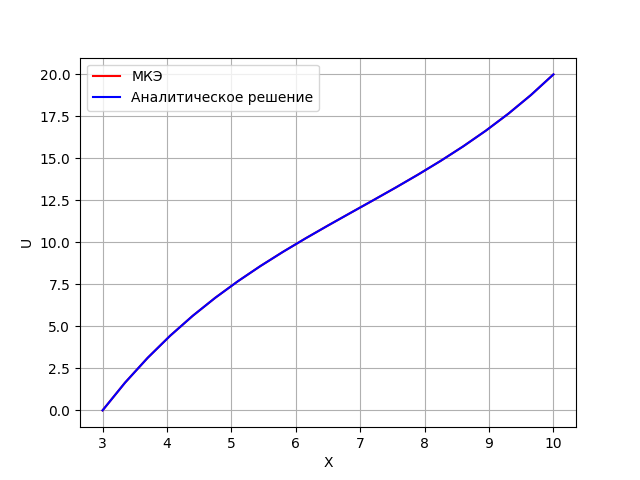
\includegraphics[width=1\textwidth]{labs/img/cub/20.png} % первое изображениие
        \caption{Результат работы программы для 20 КЭ}
        \label{c_20}
    \end{minipage}\hfill
    \begin{minipage}{0.5\textwidth}
        \centering
        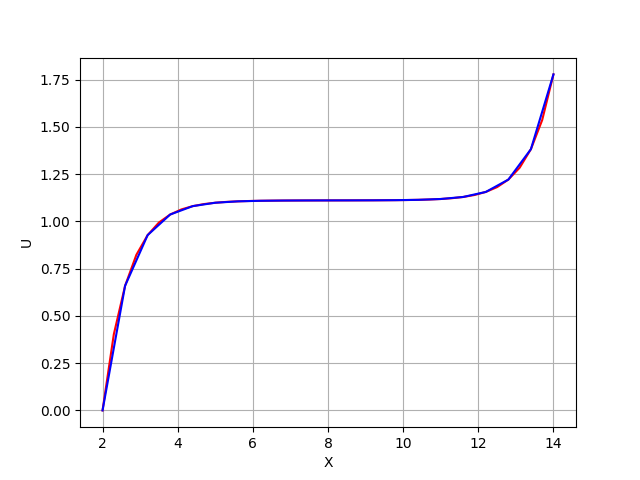
\includegraphics[width=1\textwidth]{labs/img/cub/40.png} % второе изображение
        \caption{Результат работы программы для 40 КЭ}
        \label{c_40}
    \end{minipage}
\end{figure}

\begin{table}[H]
\centering
\begin{tabular}{|c|c|c|c|}
\hline
X & Аналитическое & МКЭ-    & Абсолютная \\
  & решение       & решение & погрешность \\
\hline
\input{labs/text/tab/cub_20.txt} \\
\hline
\end{tabular}
\caption{20 кубических КЭ}
\label{table:lin_20}
\end{table}

\begin{table}[H]
\centering
\begin{tabular}{|c|c|c|c|}
\hline
X & Аналитическое & МКЭ-    & Абсолютная \\
  & решение       & решение & погрешность \\
\hline
\input{labs/text/tab/cub_40.txt} \\
\hline
\end{tabular}
\caption{40 кубических КЭ}
\label{table:lin_40}
\end{table}

Максимальная абсолютная погрешность \input{labs/text/pgr/cub_20.txt} и \input{labs/text/pgr/cub_40.txt} соответственно.


\subsubsection{Нахождение количества линейных КЭ, обеспечивающих ту же точность, что и 20 кубических}

Так как очевидно, что при увлечении числа КЭ точность растет, найдем искомое следуя алгоритму, представленному на рисунке \ref{alg}.

\begin{figure}[H]
\centerline{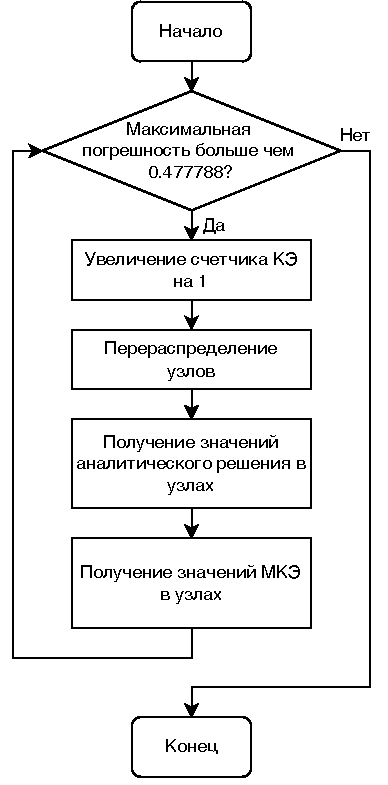
\includegraphics[scale = 0.65]{labs/img/img2.pdf}}
\caption{Алгоритм нахождения количества КЭ, заданную точность}
\label{alg}
\end{figure}

Реализовав данный алгоритм с начальным количеством КЭ=20 и увеличивая счетчик всегда на 1 получаем необходимое количество КЭ, равное \input{labs/text/pogr.txt}.

\subsection{Код}

\begin{lstlisting}[language=c++, label=prog,caption={\textit{Реализация МКЭ}}]

	#include <iostream>
#include <vector>
#include <cmath>

double EPS = 1e-16;
double X_BEGIN = 3.0;
double X_END = 14.0;
size_t ELEMS_NUM = 20;
double L = (X_END - X_BEGIN) / ELEMS_NUM;

double a = 1.0, B = 0.0, C = -15.0, D = 4.0, usl_left = 10.0, usl_right = 1.0; // au"+Bu'+Cu+D=0

std::vector<double> solve_with_gauss(std::vector<std::vector<double>>& A, std::vector<double>& b){
    size_t row_size = A.size();
    size_t col_size = A.back().size();

    // Прямой ход Гаусса
    double pivot = 0.;
    for (size_t i = 0; i < row_size; i++) {
        for (size_t j = i + 1; j < col_size; j++) {
            if (std::abs(A.at(j).at(i)) < EPS) {
                continue;
            }
            pivot = A.at(j).at(i) / A.at(i).at(i);
            b.at(j) -= pivot * b.at(i);
            for (size_t k = 0; k < row_size; k++) {
                A.at(j).at(k) -= pivot * A.at(i).at(k) ;
            }
        }
    }

    // Обратный ход Гаусса
    std::vector<double> x(row_size);
    for (int i = row_size - 1.; i >= 0; i--) {
        x.at(i) = b.at(i);
        for (size_t j = i + 1; j < row_size; j++) {
            x.at(i) -= x.at(j) * A.at(i).at(j);
        }
        x.at(i) /= A.at(i).at(i);
    }

    return x;
}

double analytical_solution(double x) {
    return (exp(-sqrt(15.) * (x + 3.)) * (146. * exp(2. * sqrt(15.) * x) + 4. * exp(sqrt(15.) * (x + 3.)) + 4. * exp(sqrt(15.) * (x + 25.)) + sqrt(15) * exp(sqrt(15.) * (2. * x + 11.)) - sqrt(15.) * exp(17. * sqrt(15.)) + 146. * exp(28. * sqrt(15.)))) / (15. * (1. + exp(22. * sqrt(15.))));
}

std::vector<double> build_analytical_solution(std::vector<double>& x_vec) {
    size_t x_vec_size = x_vec.size();
    std::vector<double> y_vec = std::vector<double>(x_vec_size);
    for (size_t i = 0; i < x_vec_size; i++) {
        y_vec.at(i) = analytical_solution(x_vec.at(i));
    }
    return y_vec;
}

std::vector<double> build_linear_solution(size_t elems_num) {
    double L = (X_END - X_BEGIN) / elems_num;
    size_t size = elems_num + 1;
    std::vector< std::vector<double> > A(size, std::vector<double>(size));
    std::vector<double> b(size);

    // Локальная матрица жесткости для линейного КЭ
    std::vector< std::vector<double> > local_matrix = {
        { a/L - C * L/3.0 + B*1.0/2.0, -a/L - C * L/6.0 - B*1.0/2.0},
        { -a/L - C * L/6.0 + B*1.0/2.0, a/L - C*L/3.0 - B*1.0/2.0},
    };

    // Ансамблирование и получение глобальной матрицы жесткости для линейного КЭ
    for (size_t i = 0; i < elems_num; i++) {
        for (size_t j = 0; j < 2; j++) {
            for (size_t k = 0; k < 2; k++) {
                A.at(i + j).at(i + k) += local_matrix.at(j).at(k);
            }
        }
    }

    for (size_t i = 0; i < size ; i++) {
        b.at(i) = D * L;
    }

    // Учет ГУ
    if ( 0 == 1 ) {
        b.at(0) =  D * L /2. - a*usl_left;
    } else {
        b.at(0) = usl_left;
        A.at(0).at(0) = 1;
        A.at(0).at(1) = 0;
    }

    if ( 1 == 1 ) {
        b.at(size - 1) =  D * L /2. + a*usl_right;
    } else {
        b.at(size - 1) = usl_right;
        A.at(size - 1).at(size - 1) = 1;
        A.at(size - 1).at(size - 2) = 0;
    }

    // Решение полученной СЛАУ методом Гаусса
    std::vector<double> res = solve_with_gauss(A, b);
    return res;
}

std::vector<double> build_cube_solution(size_t elems_num) {
    double L = (X_END - X_BEGIN) / elems_num;
    size_t size = elems_num + 1;
    std::vector< std::vector<double> > A(size,std::vector<double>(size));
    std::vector<double> b(size);
    
    // Локальная матрица жесткости для кубического КЭ
    std::vector< std::vector<double> > local_matrix = {
        {  a*37.0/(10.0*L) - C*8*L/105.0 +B*1.0/2.0,    -a*189.0/(40.0*L) - C*33*L/560.0 - B*57/80.0, a*27.0/(20.0*L) + C*3*L/140.0 + B*3.0/10.0, -a*13.0/(40.0*L) -  C*19.0*L/1680.0 - B*7/80.0},
        { -a*189.0/(40.0*L) - C*33*L/560.0 + B*57/80.0,  a*54.0/(5.0*L)-C*27*L/70.0,                  -a*297.0/(40*L) + C*27*L/560.0 - B*81.0/80.0,    a*27.0/(20.0*L) +  C*3*L/140.0 + B*3.0/10.0},
        {  a*27.0/(20.0*L) + C*3*L/140.0 - B*3.0/10.0,  -a*297.0/(40.0*L) + C*27*L/560.0 + B*81.0/80.0,  a*54.0/(5.0*L) - C*27*L/70.0,                -a*189.0/(40.0*L) - C*33*L/560.0 - B*57/80.0},
        { -a*13.0/(40.0*L) - C*19.0*L/1680.0 + B*7/80.0,   a*27.0/(20.0*L) + C*3*L/140.0 - B*3.0/10.0 , -a*189.0/(40.0*L) - C*33*L/560.0 + B*57/80.0,      a*37.0/(10.0*L) - C*8*L/105.0 - B*1.0/2.0}

    };

    
    // Локальный вектор нагрузок (дополнительные слагаемые для первого и последнего элементов учитываются далее)
    std::vector<double> local_b = { D * L / 8.0,
                                    D * 3.0 * L / 8.0,
                                    D * 3.0 * L / 8.0,
                                    D * L / 8.0 };

    
    // Производим матричные преобразования для обнуления элементов локальной матрицы жесткости, относящихся к внутренним узлам
    for (size_t i = 1; i < 3; i++) {
        for (size_t j = 0; j < 4; j++) {
            if (std::fabs(local_matrix.at(j).at(i)) > EPS && i != j) {
                double  val = local_matrix.at(j).at(i) /local_matrix.at(i).at(i);
                local_b.at(j) -= val * local_b.at(i);
                for (size_t k = 0; k < 4; k++) {
                    local_matrix.at(j).at(k) -= val *local_matrix.at(i).at(k);
                }
            }
            continue;
        }
    }
    
    
    // Исключаем внутренние узлы из рассмотрения
    std::vector< std::vector<double> >  local_matrix_mod  = { { local_matrix.at(0).at(0), local_matrix.at(0).at(3) },
                                                              { local_matrix.at(3).at(0), local_matrix.at(3).at(3) } };
    std::vector<double> local_b_mod = { local_b.at(0), 
                                        local_b.at(3)
                                        };
    
    // Ансамблирование и получение глобальной матрицы жесткости для кубического КЭ
    for (size_t i = 0; i < elems_num; i++) {
        for (size_t j = 0; j < 2; j++) {
            for (size_t k = 0; k < 2; k++) {
                A.at(i + j).at(i + k) += local_matrix_mod.at(j).at(k);
            }
        }
    }

    for (size_t i = 0; i < elems_num; i++) {
        b.at(i) += local_b_mod.at(0);
        b.at(i+1) += local_b_mod.at(1);
    }
       
    // Учет ГУ
    if (0 == 1 ) {
        b.at(0) =  local_b_mod.at(0) - a * usl_left;
    } else {
        b.at(0) = usl_left;
        A.at(0).at(0) = 1.;
        A.at(0).at(1) = 0.;
    }

    if (1 == 1 ) {
        b.at(size - 1) =  local_b_mod.at(1) + a * usl_right;
    } else {
        b.at(size - 1) = usl_right;
        A.at(size - 1).at(size - 1) = 1.;
        A.at(size - 1).at(size - 2) = 0.;
    }
    
    // Решение полученной СЛАУ методом Гаусса
    std::vector<double> res = solve_with_gauss(A, b);
    return res;
}

double calc_abs_error(const std::vector<double>& y_real, const std::vector<double>& y) {
    double max_err = 0.0;
    for (size_t i = 0; i < y_real.size(); i++) {
        double err = std::fabs(y_real.at(i) - y.at(i));
        if (err > max_err) {
            max_err = err;
        }
    }
    return max_err;
}

int main() {

     std::vector<double> x(ELEMS_NUM + 1);
     for (size_t i = 0; i < x.size(); i++) {
         x.at(i) = X_BEGIN + i * L;
     }
     size_t x_size = x.size();

    std::vector<double> y;
    if (true) {
        y = build_linear_solution(ELEMS_NUM);
    } else {
        y = build_cube_solution(ELEMS_NUM);
    }
     std::vector<double> y_real = build_analytical_solution(x);
    

     FILE* gp;
     FILE* ab;
     FILE* pgr;
     FILE* tab;
     if (true) {
        if(ELEMS_NUM == 20) {
            gp = fopen("res/labs/text/graph/lin_20.txt", "w");
            ab = fopen("res/labs/text/graph/abs.txt", "w");
            for (size_t i = 0; i < x_size; i++) {
                fprintf(ab, "%lf %lf\n", x.at(i), y_real.at(i));
            }
            pgr = fopen("res/labs/text/pgr/lin_20.txt", "w");
            tab = fopen("res/labs/text/tab/lin_20.txt", "w");
        }
        if(ELEMS_NUM == 40) {
            gp = fopen("res/labs/text/graph/lin_40.txt", "w");
            pgr = fopen("res/labs/text/pgr/lin_40.txt", "w");
            tab = fopen("res/labs/text/tab/lin_40.txt", "w");
        }
     } else {
        if(ELEMS_NUM == 20) {
            gp = fopen("res/labs/text/graph/cub_20.txt", "w");
            pgr = fopen("res/labs/text/pgr/cub_20.txt", "w");
            tab = fopen("res/labs/text/tab/cub_20.txt", "w");
        }
        if(ELEMS_NUM == 40) {
            gp = fopen("res/labs/text/graph/cub_40.txt", "w");
            pgr = fopen("res/labs/text/pgr/cub_40.txt", "w");
            tab = fopen("res/labs/text/tab/cub_40.txt", "w");
        }
     }

     for (size_t i = 0; i < x.size()-1; i++) {
        fprintf(tab, "%lf & %lf & %lf & %lf \\\\\n", x.at(i), y_real.at(i), y.at(i), std::fabs(y_real.at(i) - y.at(i)));
     }
     fprintf(tab, "%lf & %lf & %lf & %lf", x.at(x.size()-1), y_real.at(x.size()-1), y.at(x.size()-1), std::fabs(y_real.at(x.size()-1) - y.at(x.size()-1)));

     for (size_t i = 0; i < x_size; i++) {
         fprintf(gp, "%lf %lf\n", x.at(i), y.at(i));
     }

     fprintf(pgr, "%e", calc_abs_error(y_real, y));
     fclose(gp);
     fclose(ab);
     fclose(pgr);
     fclose(tab);

     return 0;
}

\end{lstlisting}
%-------------------------------------------------
\subsection{Вывод}

В ходе выполнения лабораторной работы был реализован МКЭ для различных функций форм, а также найдено количество линейных КЭ обеспечивающих точность 20ти кубических КЭ.

% --------------------------------------
% Атрибуты задачи
\labattributes{}{}{}{}{студент группы \EduGroup, \Author}{\Year, \Semestr}
%--------------

%   +1 
%   -1 

%  
%  

%   +4 
%   -4 